\documentclass[aspectratio=169,12pt]{beamer}
\usepackage[T1]{fontenc}\usepackage[utf8]{inputenc}
\usepackage{lmodern,microtype,booktabs,tabularx,tikz,pgfplots}
\usetikzlibrary{arrows.meta,positioning,fit}
\pgfplotsset{compat=1.18}
\definecolor{ink}{HTML}{202722}\definecolor{accent}{HTML}{426B52}
\definecolor{paper}{HTML}{FAFAF6}
\setbeamercolor{normal text}{fg=ink,bg=paper}
\setbeamercolor{frametitle}{fg=ink}
\setbeamercolor{structure}{fg=accent}
\setbeamertemplate{navigation symbols}{}
\setbeamertemplate{itemize item}{\small\raise.15ex\hbox{\textbullet}}
\setbeamersize{text margin left=.8cm,text margin right=.8cm}
\setbeamerfont{frametitle}{size=\fontsize{23}{26},series=\bfseries}
\setbeamertemplate{frametitle}{\vspace{.38cm}\insertframetitle\par\vspace{.12cm}}
\setbeamertemplate{footline}{\hspace{.8cm}\raisebox{.23cm}{\scriptsize MLOps Endesa | M4--M6 | DRAFT}\hfill\raisebox{.23cm}{\scriptsize\insertframenumber/16}\hspace{.8cm}}
\newcommand{\repo}{https://github.com/mlops-2627q1-mds-upc/MLOps_Endesa}
\newcommand{\candidate}{f9b5896af998331494175733c557e8dc5dd12cc7}
\newcommand{\chartheight}{4.4cm}
\newcommand{\source}[2]{\par\vspace{.15cm}{\scriptsize Source: \href{\repo/blob/\candidate/#1}{#2}\par}}
\newcommand{\bigfact}[1]{{\fontsize{36}{39}\selectfont\bfseries #1}}
\input{data-values.tex}
\title{From a selected model to a reviewable release}
\author{Team MLOps Endesa}\date{Final presentation draft | 12 November 2026}
\begin{document}
\begin{frame}[plain]
{\large UPC MDS | MLOps | Milestones 4--6}\par\vspace{.65cm}
{\fontsize{31}{35}\selectfont\bfseries From a selected model\\to a reviewable release\par}
\vspace{.4cm}
Deployment, CI/CD and monitoring\par\vspace{.4cm}
{\small Sindri Másson | Dídac Cayuela | Pablo Pérez\\Pau Adal | Antoni Lopera}\par\vspace{.35cm}
{\small DRAFT | Integrated candidate \href{\repo/pull/100}{PR \#100}, open}\par
{\small Human review and final release execution remain pending.}
\end{frame}

\begin{frame}{One forecast contract connects every layer}
\begin{columns}[T]
\begin{column}{.56\textwidth}
\bigfact{512 $\rightarrow$ 48}\par\vspace{.3cm}
Past demand positions become next-day forecasts for five states.
\end{column}
\begin{column}{.38\textwidth}
Selected model test MASE\par\vspace{.18cm}\bigfact{0.5571}\par
{\small Historical comparison; test block consumed.}
\end{column}
\end{columns}
\vspace{.5cm}
Source scale and positional time remain explicit.\par
No verified civil-clock mapping or operational-grid claim.
\source{docs/MODEL_CARD.md}{Model and dataset cards; Experiment 004}
\end{frame}

\begin{frame}{Inference, replay and service signals stay separate}
\vspace{.4cm}
\resizebox{\linewidth}{!}{%
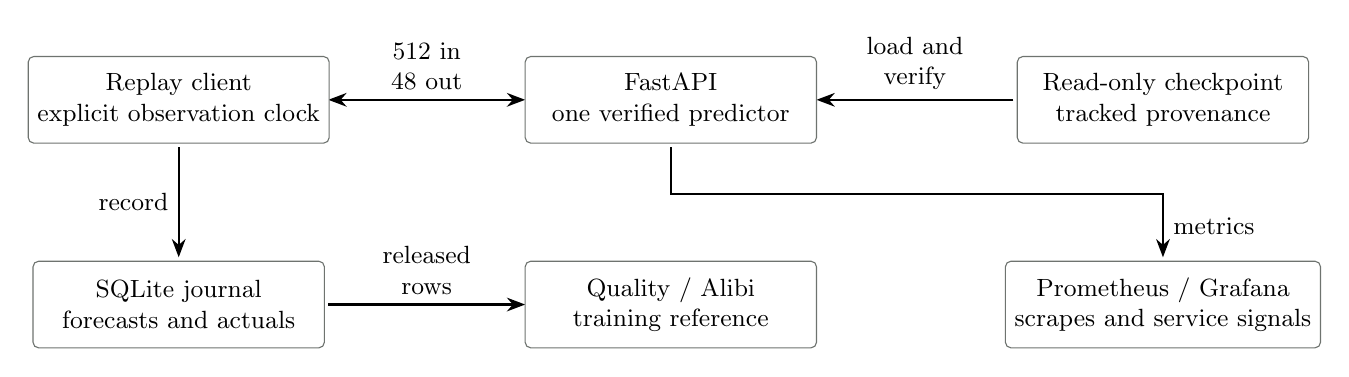
\begin{tikzpicture}[font=\small,>=Stealth,
  box/.style={draw=ink!65,rounded corners=2pt,align=center,minimum width=3.7cm,minimum height=1.1cm,fill=white}]
\draw[<->,thick] (1.9,0) -- node[above,align=center]{512 in\\48 out} (4.4,0);
\draw[->,thick] (10.6,0) -- node[above,align=center]{load and\\verify} (8.1,0);
\draw[->,thick] (0,-.6) -- node[left]{record} (0,-2.0);
\draw[->,thick] (1.9,-2.6) -- node[above,align=center]{released\\rows} (4.4,-2.6);
\draw[->,thick] (6.25,-.6) -- (6.25,-1.2) -- (12.5,-1.2) -- node[right]{metrics} (12.5,-2.0);
\node[box] at (0,0) {Replay client\\explicit observation clock};
\node[box] at (6.25,0) {FastAPI\\one verified predictor};
\node[box] at (12.5,0) {Read-only checkpoint\\tracked provenance};
\node[box] at (0,-2.6) {SQLite journal\\forecasts and actuals};
\node[box] at (6.25,-2.6) {Quality / Alibi\\training reference};
\node[box] at (12.5,-2.6) {Prometheus / Grafana\\scrapes and service signals};
\end{tikzpicture}}

\vspace{.3cm}
{\small Implemented architecture in the candidate; final target execution is pending.}
\source{docs/monitoring-scenarios.md}{API, replay, quality, drift and service contracts}
\end{frame}

\begin{frame}{A healthy process is only one check}
\renewcommand{\arraystretch}{1.35}
\begin{tabularx}{\linewidth}{lX}
\textbf{200 /health} & Process responds.\\
\textbf{200 /ready} & Verified predictor is loaded.\\
\textbf{200 /forecast} & 48 finite, ordered quantiles and actual model/settings.\\
\textbf{422 invalid input} & Strict state, numeric type and history-length contract.\\
\end{tabularx}
\vspace{.3cm}
Missing weights abort startup. Prediction failure returns 503.\par
The service has no model fallback or training endpoint.
\source{docs/api.md}{Merged API PR \#86; historical model smoke is separate}
\end{frame}

\begin{frame}{The image carries code; the mount carries weights}
\begin{columns}[T]
\begin{column}{.48\textwidth}
{\large\bfseries Immutable runtime}\par\vspace{.2cm}
Pinned base images\par
Locked CPU serving group\par
UID 10001, one worker\par
No data, weights or credentials
\end{column}
\begin{column}{.44\textwidth}
{\large\bfseries Verified model slot}\par\vspace{.2cm}
Read-only checkpoint + params\par
Weight-bound training provenance\par
Two numerical threads\par
Mismatch fails startup
\end{column}
\end{columns}
\vspace{.5cm}
Native-amd64 CI uses a synthetic factory.\par
Independent selected-model image startup remains pending.
\source{docs/container.md}{Pending PR \#88; fixture-only container workflow}
\end{frame}

\begin{frame}{Release evidence must match the exact source}
\vspace{.2cm}
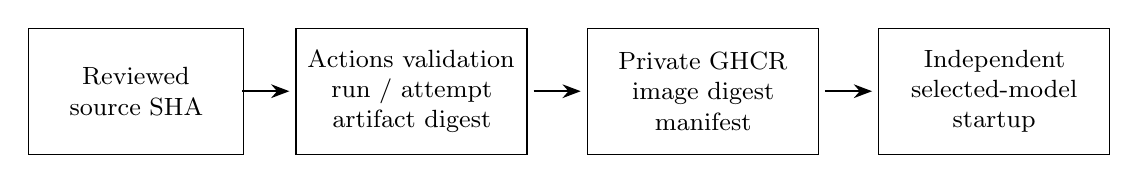
\begin{tikzpicture}[x=1cm,y=1cm,font=\small,>=Stealth]
\draw[->,thick] (2.5,0)--(3.1,0);
\draw[->,thick] (6.2,0)--(6.8,0);
\draw[->,thick] (9.9,0)--(10.5,0);
\node[draw,align=center,minimum height=1.6cm,text width=2.5cm] at (1.15,0){Reviewed\\source SHA};
\node[draw,align=center,minimum height=1.6cm,text width=2.7cm] at (4.65,0){Actions validation\\run / attempt\\artifact digest};
\node[draw,align=center,minimum height=1.6cm,text width=2.7cm] at (8.35,0){Private GHCR\\image digest\\manifest};
\node[draw,align=center,minimum height=1.6cm,text width=2.7cm] at (12.05,0){Independent\\selected-model\\startup};
\end{tikzpicture}
\par
\vspace{.5cm}
A changed commit requires matching validation.\par
First publication is explicit and default-off; 404 is UNOBSERVED.
\source{docs/image-publication.md}{PRs \#87/\#98; no publication executed}
\end{frame}

\begin{frame}{Recovery preserves the accepted baseline}
\begin{enumerate}
\item Lock the persistent state; check expected-current identity.
\item Verify the baseline forecast; persist pending release identities.
\item Require a clean stop, then start and check the candidate.
\item On failure, restore the baseline and observe another forecast.
\end{enumerate}
\vspace{.3cm}
{\large Candidate failure stays a failed attempt, even after recovery.}\par
\vspace{.2cm}
{\small Source/fixture behaviour is implemented. Final target rollback is pending.}
\source{docs/deployment-release.md}{PR \#99; recorded status alone is not target health}
\end{frame}

\begin{frame}{Green CI establishes a bounded source result}
\begin{columns}[T]
\begin{column}{.42\textwidth}
\bigfact{1,037}\par
Tests passed\par\vspace{.25cm}
109 skipped | 82\% coverage
\end{column}
\begin{column}{.52\textwidth}
Required lint/test\par
Workflow semantics\par
Native-amd64 container fixture\par
Service/promtool checks\par
Separate actual synthetic Alibi
\end{column}
\end{columns}
\vspace{.5cm}
{\small All seven applicable checks passed for PR \#100's exact head.\par
GitHub's generated merge checkout is a separate recorded identity.\par
This result does not establish publication, peer approval or deployment.}
\source{docs/release-validation.md}{\#100 Actions records, linked in the final source ledger}
\end{frame}

\begin{frame}{More concurrency increased delay, not throughput}
\begin{columns}[c]
\begin{column}{.66\textwidth}
\begin{tikzpicture}
\begin{axis}[width=.94\linewidth,height=\chartheight,ymin=0,ymax=11,
  ybar,bar width=24pt,xtick={0,1},xticklabels={Concurrency 1,Concurrency 2},
  ylabel={Warm p95 (seconds)},ytick={0,2,4,6,8,10},
  xmin=-.6,xmax=1.6,axis x line*=bottom,axis y line*=left,
  ymajorgrids=true,grid style={gray!20},
  tick label style={font=\small},label style={font=\small},
  legend columns=2,
  legend style={font=\small,draw=none,at={(.5,1.02)},anchor=south},
  nodes near coords,nodes near coords style={font=\small,/pgf/number format/fixed,/pgf/number format/precision=2}]
\addplot[fill=ink!80,draw=ink!80] table[x=index,y=discovery,col sep=comma]{latency.csv};
\addplot[fill=accent!65,draw=accent] table[x=index,y=confirmation,col sep=comma]{latency.csv};
\legend{Discovery,Confirmation}
\end{axis}
\end{tikzpicture}

\end{column}
\begin{column}{.29\textwidth}
\bigfact{94}\par
Forecasts, zero HTTP errors\par\vspace{.2cm}
{\small About 0.22 requests/s.\par
20 warm requests per phase; one VM/input.}
\end{column}
\end{columns}
{\small Historical 2 November experiment. No adopted latency SLO; final image pending.}
\source{docs/experiments/009-serving-benchmark.md}{Recorded discovery and confirmation; PR \#93}
\end{frame}

\begin{frame}{An isolated outage fired and cleared a real alert}
\resizebox{.98\linewidth}{!}{%
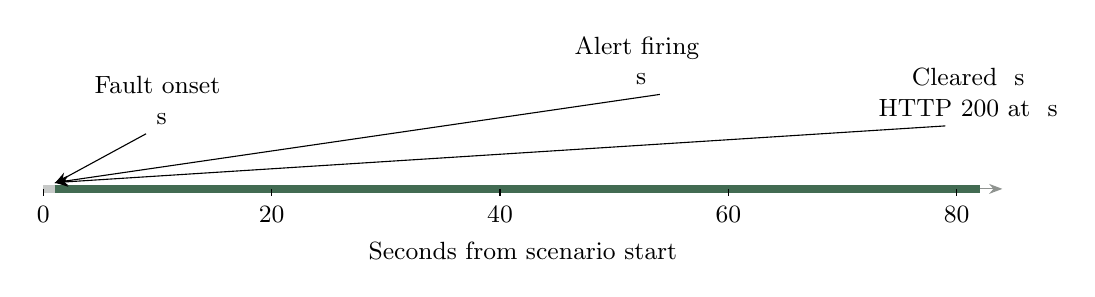
\begin{tikzpicture}[x=.145cm,y=1cm,font=\small,>=Stealth]
\draw[->,ink!50] (0,0) -- (84,0);
\draw[line width=3pt,ink!25] (0,0) -- (\OutageStart,0);
\draw[line width=3pt,orange!65!black] (\OutageStart,0) -- (\OutageFire,0);
\draw[line width=3pt,red!65!black] (\OutageFire,0) -- (\OutageClear,0);
\draw[line width=3pt,accent] (\OutageClear,0) -- (82,0);
\foreach \x in {0,20,40,60,80}{\draw (\x,0) -- (\x,-.09);\node[below] at (\x,-.1){\x};}
\node[below] at (42,-.55){Seconds from scenario start};
\draw[->] (9,.7) -- (\OutageStart,.07);
\node[above,align=center] at (10,.7){Fault onset\\\OutageStart{} s};
\draw[->] (54,1.2) -- (\OutageFire,.08);
\node[above,align=center] at (52,1.2){Alert firing\\\OutageFire{} s};
\draw[->] (79,.8) -- (\OutageClear,.08);
\node[above,align=center] at (81,.8){Cleared \OutageClear{} s\\HTTP 200 at \OutageHttp{} s};
\end{tikzpicture}}

\OutageDelay{} seconds from fault onset to firing.\par
{\small One-minute hold unchanged. Local synthetic API + real Prometheus;\par
amd64 emulation on Mac. No external receiver is configured.}
\source{monitoring/scenarios/local-evidence-2026-11-12.json}{Fresh \#84 local observation; final target remains pending}
\end{frame}

\begin{frame}{Delayed truth must remain visibly pending}
\begin{columns}[T]
\begin{column}{.45\textwidth}
{\large Replay clock 516}\par\vspace{.2cm}
\bigfact{6 / 186}\par
Matched / pending steps
\end{column}
\begin{column}{.45\textwidth}
{\large Replay clock 563}\par\vspace{.2cm}
\bigfact{192 / 0}\par
Matched / pending steps
\end{column}
\end{columns}
\vspace{.5cm}
Default minimum-30 horizon groups still lack enough samples.\par
{\small Synthetic display minimum: two. Missing truth never becomes zero error.}
\source{docs/monitoring-scenarios.md}{Fresh public journal/quality/exporter scenario}
\end{frame}

\begin{frame}{The sampled 80\% interval was under-covered}
\begin{columns}[c]
\begin{column}{.66\textwidth}
\begin{tikzpicture}
\begin{axis}[width=.94\linewidth,height=\chartheight,ymin=0,ymax=100,
  ybar,bar width=22pt,xtick={0,1,2,3,4},xticklabels={NSW,VIC,QLD,SA,TAS},
  ylabel={Empirical coverage (\%)},ytick={0,20,40,60,80,100},
  xmin=-.6,xmax=4.6,axis x line*=bottom,axis y line*=left,
  ymajorgrids=true,grid style={gray!20},tick label style={font=\small},
  label style={font=\small},enlarge x limits=false]
\addplot[fill=accent,draw=accent,point meta=y,nodes near coords,
 nodes near coords style={font=\small,/pgf/number format/fixed,/pgf/number format/precision=1}]
 table[x=index,y=coverage,col sep=comma]{coverage.csv};
\addplot[sharp plot,dashed,thick,ink,forget plot] coordinates {(-.6,80) (4.6,80)};
\node[anchor=south east,font=\small] at (axis cs:4.55,82) {Nominal 80\%};
\end{axis}
\end{tikzpicture}

\end{column}
\begin{column}{.29\textwidth}
\bigfact{30}\par
Validation origins / state\par\vspace{.25cm}
{\small 150 forecasts\par 7,200 matched steps\par
No full-block calibration or coverage SLO.}
\end{column}
\end{columns}
\source{monitoring/quality/validation-subset.json}{Historical selected-model subset; pending PR \#92}
\end{frame}

\begin{frame}{Fresh KS detects the declared synthetic shift}
\renewcommand{\arraystretch}{1.6}
\begin{tabularx}{\linewidth}{lXX}
\textbf{37,632} & Control & No drift, five states\\
\textbf{40,320} & Fixed level shift & Drift, five states\\
\textbf{43,008} & Restored distribution & No drift, five states\\
\end{tabularx}
\vspace{.3cm}
{\large Each comparison needs 2,688 positional steps: 56 nominal days.}\par
\vspace{.2cm}
{\small Compressed execution time is not live detection latency.\par
The next statistical result is not notification delivery or an operational reset.}
\source{docs/monitoring-scenarios.md}{Actual fresh Alibi 0.13.0; separate from historical playback}
\end{frame}

\begin{frame}{Retained limitations change what we can claim}
\begin{tabularx}{\linewidth}{lX}
\textbf{8 / 30} & Historical drift control alarms; natural changes may exist.\\[.3cm]
\textbf{56--112 days} & Historical first shift detections, with missed windows.\\[.3cm]
\textbf{Exit 137} & Historical stops had no recorded OOM; graceful stop unproven.\\[.3cm]
\textbf{Two failed runs} & Local scenario failures retained before corrected reruns.\\
\end{tabularx}
\vspace{.3cm}
Numerical operating policies need human decisions.\par
No automatic retraining or further tuning on the consumed test block.
\source{docs/drift.md}{Drift record, benchmark manifest and local scenario failures}
\end{frame}

\begin{frame}{AI supported substantive implementation and analysis}
Codex helped implement release helpers, tests, monitoring and scenarios;
reconciled evidence; wrote report/deck sources and diagrams.\par\vspace{.3cm}
Claude Code assisted earlier data validation and report drafting.\par\vspace{.3cm}
Human experimental choices and recorded reviews retain their attribution.\par
\vspace{.4cm}
{\large Final team assessment and proposed EDN acceptance remain human tasks.}
\source{docs/edn/README.md}{Merged EDNs 001--012; existing PR \#97 pending and unchanged}
\end{frame}

\begin{frame}{The next delivery step is reviewed execution}
\begin{enumerate}
\item Human review/merges and exact-source Actions model validation.
\item Private publication and independent native-amd64 startup.
\item User-provided UPC/VPN access, then fenced rollout/recovery.
\item Target monitoring, final assessments and a human rehearsal.
\end{enumerate}
\vspace{.3cm}
\textbf{DRAFT: no final release or submission is claimed.}\par
{\small Supplied schedule: report 14 December; talk 15 December.\par
Atenea changes and instructor access remain to be checked.}
\end{frame}
\end{document}
